\section{NV XY8 Case Study}

The NV-center platform is used here as a control-oriented case study of EDT-style finite-regime optimization rather than as a direct experimental realization of the materials-side curvature diagnostic~\cite{Degen2017,Barry2020}. In NV--XY8 sensing protocols, performance is governed by a structured combination of resource factors, including filter gain $G(f)$, coherence time, pulse fidelity, and readout contrast. As shown in Fig.~\ref{fig:fig5_nvdemo}, these quantities do not improve monotonically with control parameters such as pulse number $N$ or spacing $\tau$. Instead, an optimal operating point emerges as a finite regime in which signal amplification, coherence preservation, and control accuracy are balanced~\cite{Casola2018}.

This behavior is directly analogous to the EDT regime identified in the plaquette-model analysis. Increasing control strength enhances sensitivity through improved filter response, but also accelerates decoherence and accumulates control errors. As a result, sensing performance exhibits a maximum within a finite window rather than at extreme parameter values. Within this regime, the sensor dynamics remain aligned with a structured manifold in control space, enabling both selective response and coherence localization~\cite{Degen2017,Barry2020}.

\subsection{Rate-Based Model}

Quantum sensing in NV-center ensembles is analyzed within a quantum resource engineering framework using a rate-based model (\texttt{nvratemodel} API) that maps experimental control parameters to effective quantum resources and sensing performance~\cite{NVRateModel2023,Degen2017,Barry2020}. For XY8 dynamical-decoupling sequences, the control parameter set is defined as
\begin{equation}
\mathcal{C} = \{P_{\mathrm{laser}},\, t_{\mathrm{read}},\, \Omega_{\mathrm{MW}},\, \tau,\, N_{\pi},\, B_0,\, T,\, \mathrm{strain}\},
\end{equation}
which determines initialization, control, and environmental conditions of the sensor~\cite{Casola2018}.

These controls are mapped onto an effective resource vector
\begin{equation}
\mathcal{R} = \{R_{\mathrm{ph}},\, C,\, T_2(N_{\pi}),\, \chi(\omega),\, \mathrm{duty}\},
\end{equation}
where $R_{\mathrm{ph}}$ is the detected photon rate, $C$ is the fluorescence contrast, $T_2(N_{\pi})$ is the coherence time under dynamical decoupling, $\chi(\omega)$ is the filter-function response, and $\mathrm{duty}$ accounts for initialization and readout overhead. The filter function is peaked near $\omega \simeq \pi/\tau$, enabling frequency-selective amplification of ac fields~\cite{Cywinski2008}.

Sensing performance is quantified by a sensitivity proxy $\eta_{\mathrm{AC}}(\omega)$, which scales approximately as
\begin{equation}
\eta_{\mathrm{AC}}(\omega) \propto \frac{1}{\chi(\omega)\,C\,\sqrt{R_{\mathrm{ph}}\,T_2(N_{\pi})}} \times f_{\mathrm{duty}},
\end{equation}
consistent with standard analyses of NV magnetometry sensitivity~\cite{Degen2017,Barry2020}.

Parameter sweeps over $(\tau, N_{\pi})$ identify optimal sensing configurations. The resulting sensitivity landscape exhibits a finite optimum, reflecting competition between resource-enhancing mechanisms (filter gain and signal accumulation) and resource-degrading effects (decoherence, pulse errors, and overhead)~\cite{Cywinski2008,Casola2018}. This finite optimal region defines a structured manifold in control space, providing a sensing-side analog of the EDT regime.

\begin{figure*}[t]
\centering
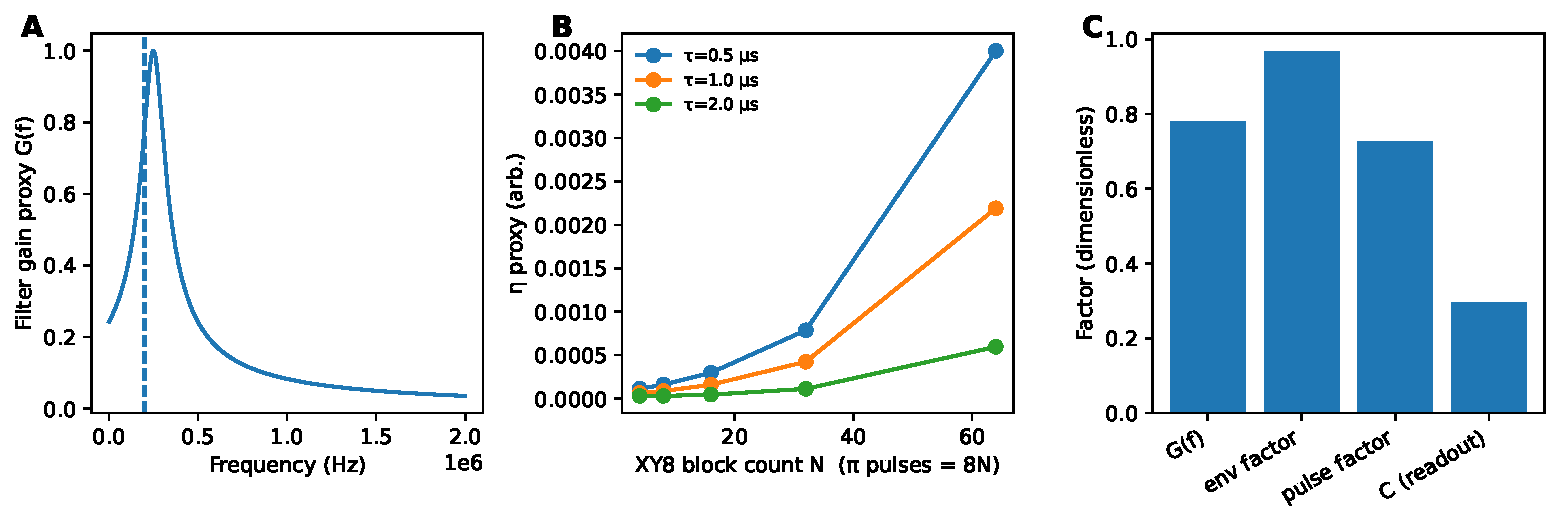
\includegraphics[width=0.90\linewidth]{fig_xy8_qre_nv.pdf}
\caption{\textbf{Quantum resource engineering in NV-center sensing.}
(A) Filter response function $G(f)$ for an XY8 sequence, showing frequency-selective amplification.
(B) Sensitivity proxy as a function of pulse number $N$ and spacing $\tau$, demonstrating a finite optimal regime.
(C) Decomposition of sensing performance into resource factors, including filter gain, environmental coherence, pulse fidelity, and readout contrast.
These results show that optimal sensing arises from a structured balance of competing quantum resources, providing a control-side case study of the EDT finite-regime logic.}
\label{fig:fig5_nvdemo}
\end{figure*}

\subsection{Cross-Platform Interpretation}

Across computation, measurement, and sensing, the same principle emerges: quantum functionality is determined by the structure of the accessible dynamical manifold rather than by the total size of Hilbert space. The plaquette model provides a minimal dynamical realization of this principle, while the NV platform demonstrates its sensing relevance. EDT therefore establishes a programmable resource framework in which control parameters define and navigate structured manifolds of useful dynamics~\cite{Preskill2018,Verstraete2008}.
